\documentclass[12pt, a4paper]{report}
\usepackage{graphicx}
\usepackage{amsmath}
\usepackage{float}
\renewcommand{\baselinestretch}{1.2} 
\usepackage{ragged2e}
\usepackage{fancyvrb}
\usepackage{amssymb}
\usepackage[a4paper, total={7in, 9in}]{geometry}
\usepackage[utf8]{inputenc}
\usepackage{physics}
\usepackage{enumitem}


\title{\textbf{EE2703 : Applied Programming Lab \\ Assignment 10 \\ Spectra of non-periodic signals }} % Title
\author{Arun Krishna A M S \\ EE19B001} % Author name
\date{2nd June 2021} % Date for the report

\begin{document}		
		
\maketitle % Insert the title, author and date
\justifying

\section*{Objective}
In the previous assignment we looked at functions that were periodic and extracted their
spectra. The approach was:
\begin{itemize}
  	\item Sample the signal so that \textbf{Nyquist Criteria} is met. Generate the frequency axis from $-f_{max}/2$ to $f_{max}/2$
    \item Obtain the \textbf{Discrete Fourier Transform}. Rotate the samples so that $f$ ranges from $f = $ $- f_{max}/2$ to $f =f_{max}/2 $ $-\Delta f$ . 
  	\item Plot the magnitude and phase of the spectrum.
\end{itemize}
In this assignment our aim is to
\begin{itemize}
  	\item Obtain and analyze the frequency response of non-periodic discrete time signals
    \item Try to minimize the errors that arise from \textbf{Gibbs Phenomenon}  by performing \textbf{Windowing} using a technique called as \textbf{Hamming} 
\end{itemize}

\section*{Analysis of Frequency Response of $\sin (\sqrt{2}t)$}
The Fast Fourier Transform any for non-periodic-function can be obtained by
\begin{verbatim}
def FastFourierTransform(function, interval, N, boolOdd):
    time = linspace(interval[0], interval[1], N + 1)[:-1]
    w = linspace(-pi*N/(interval[1]-interval[0]), 
                  pi*N/(interval[1]-interval[0]), N + 1)[:-1]
    y = function(time)
    if boolOdd == True:
        y[0] = 0
    y = fftshift(y) 
    Y = fftshift(fft(y))/N
    phase = angle(Y)
\end{verbatim}
\\

In case of function $\sin (\sqrt{2}t)$, the signal is sampled in the interval $[−\pi, \pi)$ and the \texttt{fft()} and \texttt{fftshift()} functions are used to obtain the \textbf{DFT} of the said function. 

In case of any odd function, we can observe that the code initializes the first element \texttt{y[0] = 0} to zero. This is because although the function is odd, the samples are not Anti-symmetric. Un-symmetric samples can result in residual components in phase.
\clearpage

For $i \in \{ 1,2,3... \frac{N}{2}-1 \}$:
\begin{equation*}
y[i] = y[N-i]
\end{equation*}
\begin{equation*}
y[\frac{N}{2}] = y[-t_{max}] = \sin (t_{\frac{N}{2}})
\end{equation*}
\begin{equation*}
Y[k] = \sum^{N-1}_{n = 0}y[n]exp(j \frac{2 \pi k n}{N})
\end{equation*}
\begin{equation*}
Y[k] = \sum^{\frac{N}{2}-1}_{n = 0}y[n](exp(j \frac{2 \pi k n}{N}) - exp(-j \frac{2 \pi k n}{N}) + (y[\frac{N}{2}]exp(j \pi k))
\end{equation*}
\begin{equation*}
Y[k] = \sum^{\frac{N}{2}-1}_{n = 0}-2jy[n]sin(\frac{2 \pi}{N}kn) + (-1)^k(y[\frac{N}{2}])
\end{equation*}
This system is no longer purely imaginary which is evident from \textbf{CTFT}. For the system to be purely imaginary as expected $y[0] = 0$ to give us purely imaginary phase. 

If the DFT of the function is obtained we observe the following:
\begin{center}
	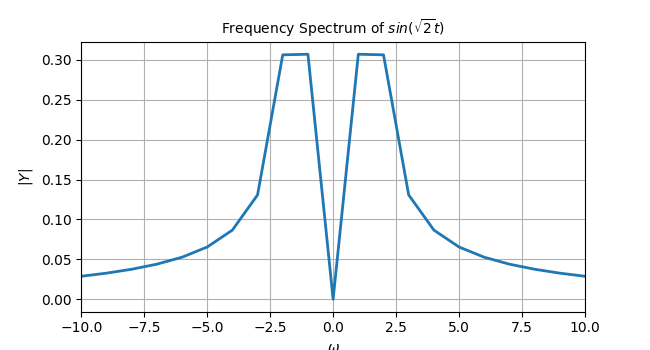
\includegraphics[scale=0.7]{Figure_1.png} 
	\label{fig:rawdata}
\end{center}
\begin{center}
	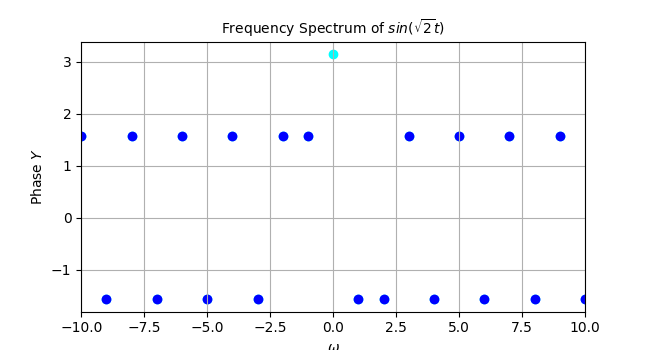
\includegraphics[scale=0.7]{Figure_2.png} 
	\label{fig:rawdata}
\end{center}
\clearpage
One could observe that frequencies are spread throughout instead of just two peaks at $ \pm \sqrt(2)$. This is because when the signal is sampled, the constructed periodic function would be
\begin{center}
	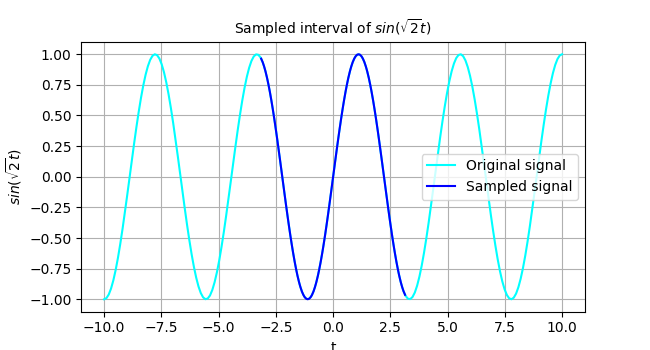
\includegraphics[scale=0.75]{Figure_3.png} 
	\label{fig:rawdata}
\end{center}
\begin{center}
	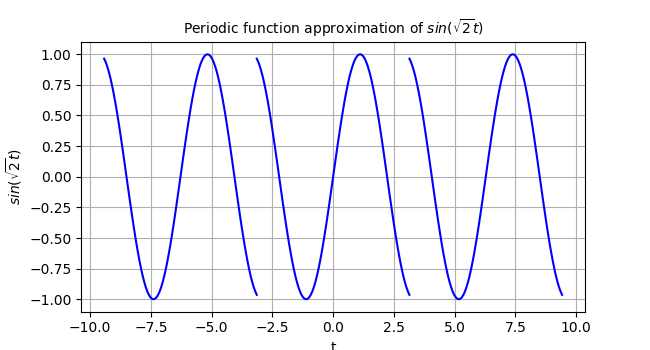
\includegraphics[scale=0.75]{Figure_4.png} 
	\label{fig:rawdata}
\end{center}
As one can observe, the periodic function of the sampled interval is not same as the original function. Even though the function $\sin (\sqrt{2}t)$ is periodic, the portion between $-\pi$ and $\pi$ is not the region that can be replicated to obtain the original periodic function. The function showed in the second graph is what the DFT is trying to fourier analyse.
\\

The discontinuities in the second graph observed for each section of 64 samples results in the \textbf{Gibbs Phenomenon}. This phenomenon results in higher frequencies having significant contributions. 

Windowing is a technique to reduce the discontinuities by damping the function near the discontinuities. For this we shall multiply the given function sequence by a \textbf{window sequence} w[n]:
\begin{equation*}
g(n) = w(n)*f(n)
\end{equation*}
This windowing will result in the spikes smeared out by $W_k$. So we expect to get broader peaks with frequencies completely suppressed at the end of the window. The function that we use for windowing is called \textbf{Hamming Window}

\begin{equation*}
f(z) =     \left\{ \begin{array}{rcl} 0.54 + 0.46 cos(\frac{2 \pi n}{N-1}) & \mbox{for}& |n| \leq \frac{N-1}{2} \\ 0  & \mbox{for} & else \end{array}\right.
\end{equation*}

The hamming function is given by
\begin{verbatim}
def sinroot2(x):
    return sin(sqrt(2) * x)

# Function to return Hamming Window sequence
def hammingFunction(n, a = 0.54,b = 0.46):
    return fftshift(a + b*cos((2*pi*n)/(len(n) - 1)))

def hammingsinroot2(x):
    return sinroot2(x)*hammingFunction(arange(len(x)))    
\end{verbatim}

After applying the hamming function one can observe that the obtained graph is
\begin{center}
	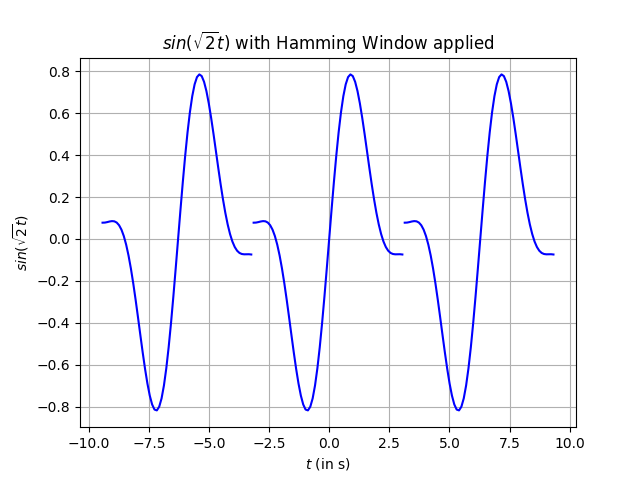
\includegraphics[scale=0.75]{Figure_5.png} 
	\label{fig:rawdata}
\end{center}
Although the function still has discontinuities, it has been greatly reduced by multiplying with the hamming function. We next try to plot the frequency spectrum of the $sin(\sqrt{2}nT_s)w[n]$ function.
\clearpage

\begin{center}
	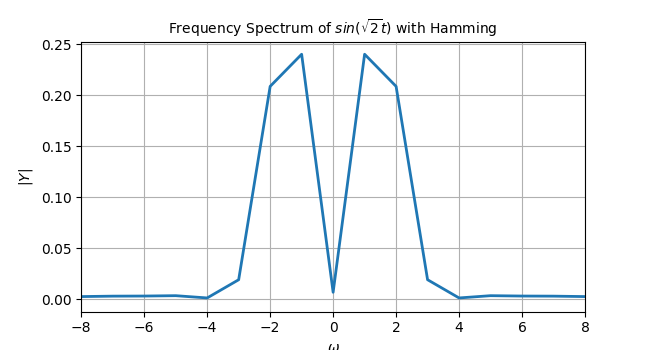
\includegraphics[scale=0.75]{Figure_6.png} 
	\label{fig:rawdata}
\end{center}
\begin{center}
	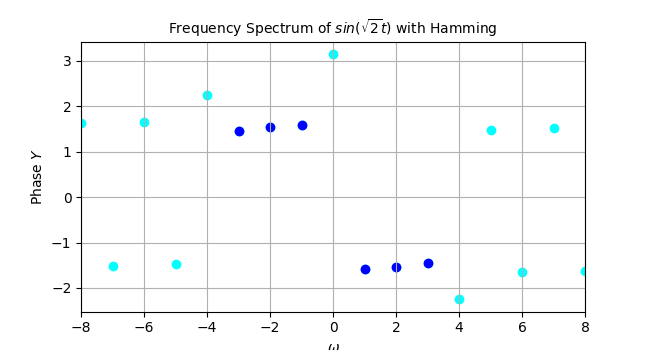
\includegraphics[scale=0.75]{Figure_7.png} 
	\label{fig:rawdata}
\end{center}

As expected the magnitude plot is closer to our expectations. But it is still too wide. We need better resolution to get better defined peaks. So we increase the time interval to $[−4 \pi, 4 \pi)$ and the samples to 256.

\begin{center}
	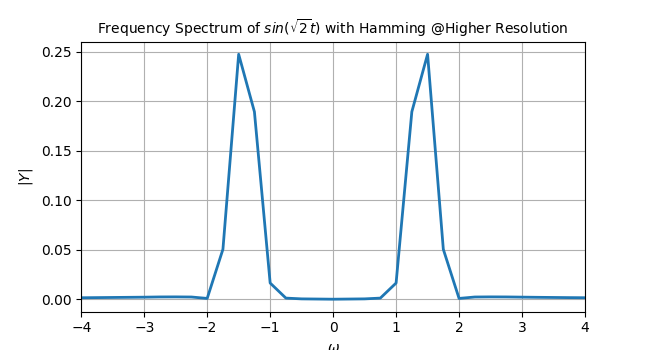
\includegraphics[scale=0.75]{Figure_8.png} 
	\label{fig:rawdata}
\end{center}
\clearpage

\begin{center}
	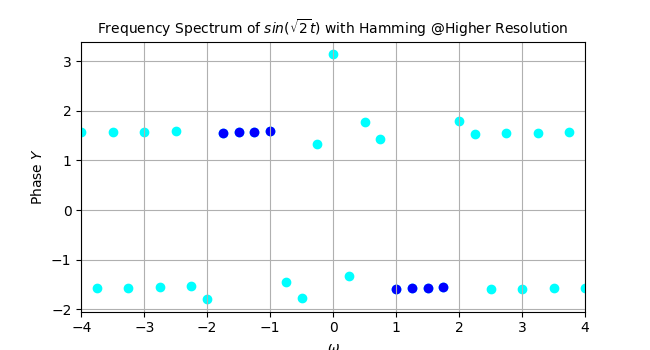
\includegraphics[scale=0.75]{Figure_9.png} 
	\label{fig:rawdata}
\end{center}
As expected the peaks are more well defined and the magnitude response falls more rapidly for higher values. But one can also observe that the width of the peaks have increased a bit with windowing for the same resolution. This is again due to windowing.


\\
\\

\section*{Analysis of Frequency Response of $\cos^3 (0.86t)$}
As before, the same procedure is applied and we observe the following for with and without hamming
\begin{center}
	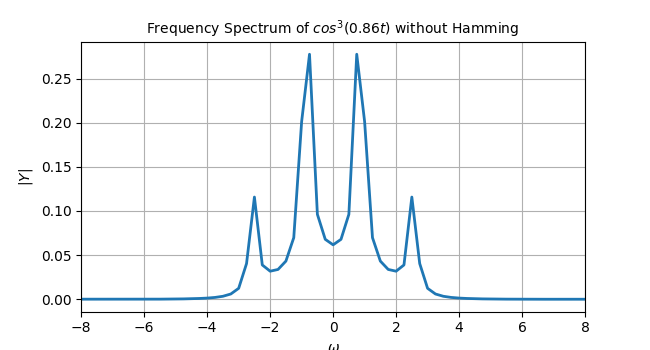
\includegraphics[scale=0.8]{Figure_10.png} 
	\label{fig:rawdata}
\end{center}
\clearpage

\begin{center}
	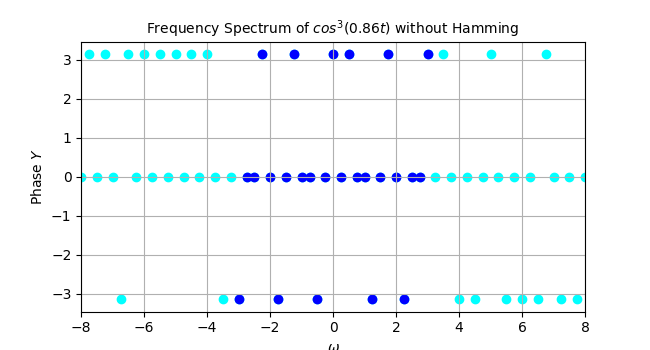
\includegraphics[scale=0.75]{Figure_11.png} 
	\label{fig:rawdata}
\end{center}
\begin{center}
	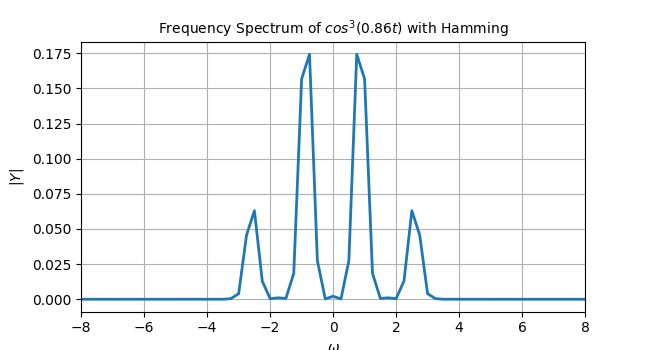
\includegraphics[scale=0.75]{Figure_12.png} 
	\label{fig:rawdata}
\end{center}
\begin{center}
	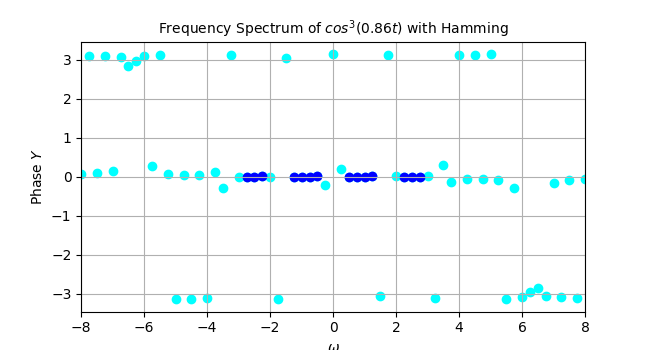
\includegraphics[scale=0.75]{Figure_13.png} 
	\label{fig:rawdata}
\end{center}
\clearpage

The graphs are expected as 
\begin{equation*}
cos^3(0.86t) = \frac{3}{4}cos(0.86t) + \frac{1}{4}cos(3(0.86t))
\end{equation*}
\begin{equation*}
cos^3(t) = \frac{3}{8}e^{0.86jt} + \frac{3}{8}e^{-0.86jt} + \frac{1}{8}e^{3(0.86)jt} + \frac{1}{8}e^{-3(0.86)jt}
\end{equation*}

We expect peaks at $0.86, -0.86, 2.58, -2.58$ frequencies which is as observed with the peaks being at approximately correct spot. The phase are also as expected equal to zero

\section*{Analysis of Frequency Response of $cos(\omega t+ \phi)$}
Next we try to find the DFT of the signal $cos(\omega t+ \phi)$ with arbitrary $\omega$ and $\phi$ values with $0.5 < \omega < 1.5$ and $-\pi < \phi < \pi$. 
\begin{equation*}
cos(\omega t+ \phi) = \frac{1}{2}e^{j \phi}e^{j \omega t} + \frac{1}{2}e^{-j \phi}e^{-j \omega t}
\end{equation*}
For this function, we observe that the peaks would lie at $\omega$ frequencies with the phase being equal to $\phi$. The following code generates an arbitrary frequency and phase and computes the function.

\begin{verbatim}
freq = random.uniform(0.5,1.5)
delta = random.uniform(-pi,pi)
def cosfunction(x):
    return cos(freq*x + delta)
\end{verbatim}

For the arbitrarily generated frequency and phase,
\begin{verbatim}
frequency =  0.5361703762348236
phase =  2.3007949240700682
\end{verbatim}

the observed frequency response is  
\begin{center}
	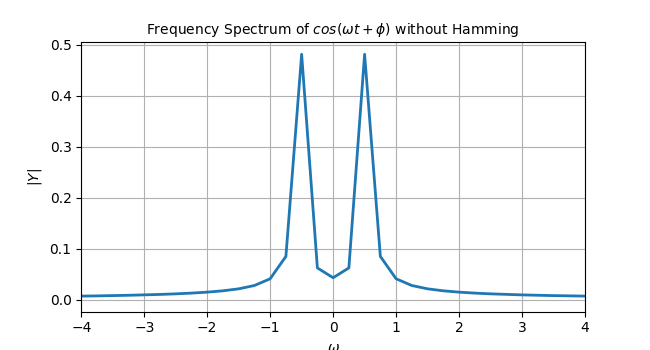
\includegraphics[scale=0.75]{Figure_14.png} 
	\label{fig:rawdata}
\end{center}
\clearpage

\begin{center}
	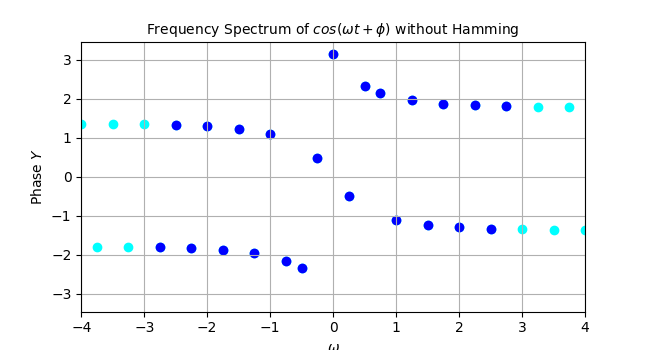
\includegraphics[scale=0.8]{Figure_15.png} 
	\label{fig:rawdata}
\end{center}

\begin{center}
	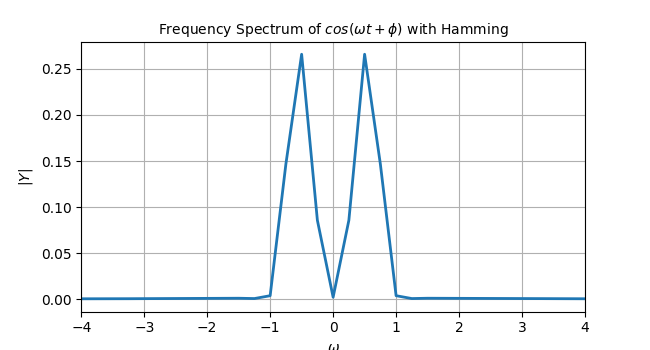
\includegraphics[scale=0.8]{Figure_16.png} 
	\label{fig:rawdata}
\end{center}

\begin{center}
	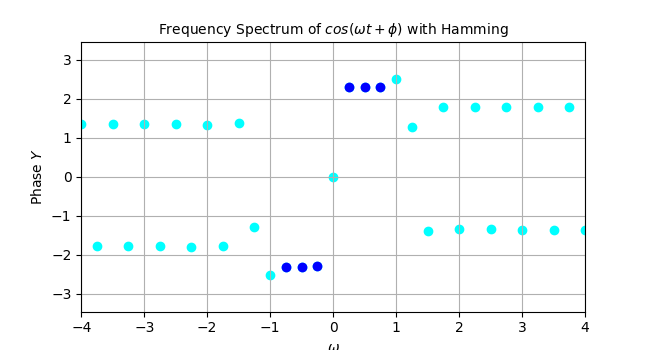
\includegraphics[scale=0.8]{Figure_17.png} 
	\label{fig:rawdata}
\end{center}
\clearpage

Suppose if we have to find the frequency $\omega$ and phase $\phi$ from the frequency response by computing a weighted average based on its magnitude. We reduce our region, by considering the magnitudes above a threshold point $(0.1)$, after which weighted average is calculated.

\begin{verbatim}
def estimatingWo_and_delta(w,mag,phase):
    significantmag = where(mag > 0.1)
    w = w[significantmag]
    mag = mag[significantmag]
    phase = phase[significantmag]
    
    estimatedWo = sum((mag**2)*abs(w))/sum(mag**2)
    estimatedDelta = sum((mag**2)*abs(phase))/sum(mag**2)    
    
    print("Estimated frequency:", estimatedWo)
    print("Estimated phase:", estimatedDelta)
\end{verbatim}

The estimated frequency and phase is
\begin{verbatim}
Estimations for cos(freq*t + phase) without hamming:
Estimated frequency: 0.5
Estimated phase: 2.3346428474376513

Estimations for cos(freq*t + phase) with hamming:
Estimated frequency: 0.5584304452185574
Estimated phase: 2.302385400626147
\end{verbatim}


\section*{Analysis of Frequency Response of $cos(\omega t+ \phi)$ with noise}
To the above signal $cos(\omega t+ \phi)$, white gaussian noise is added - after which the frequency response is again observed.
\begin{verbatim}
def noisycos(x):
    return cos(freq*x + delta) + 0.1 * randn(len(x))
\end{verbatim}
 
\clearpage
\begin{center}
	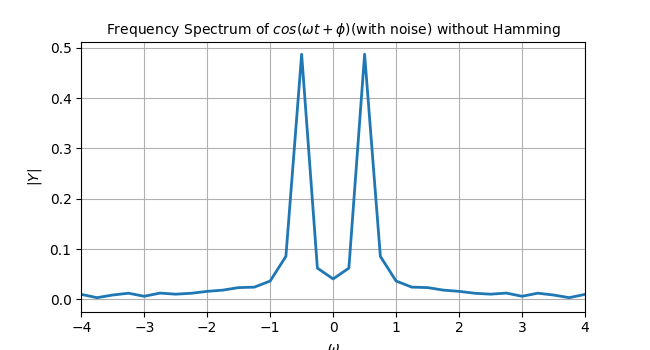
\includegraphics[scale=0.8]{Figure_18.png} 
	\label{fig:rawdata}
\end{center}
\begin{center}
	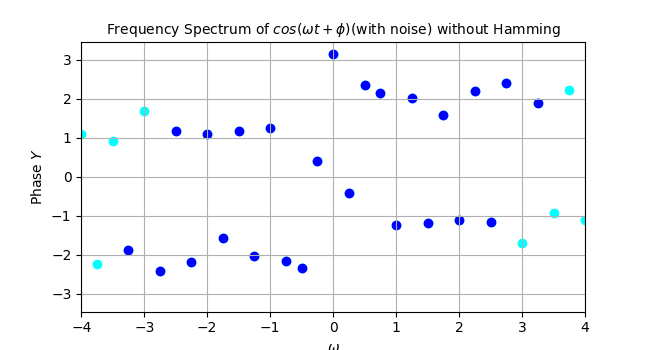
\includegraphics[scale=0.8]{Figure_19.png} 
	\label{fig:rawdata}
\end{center}
\begin{center}
	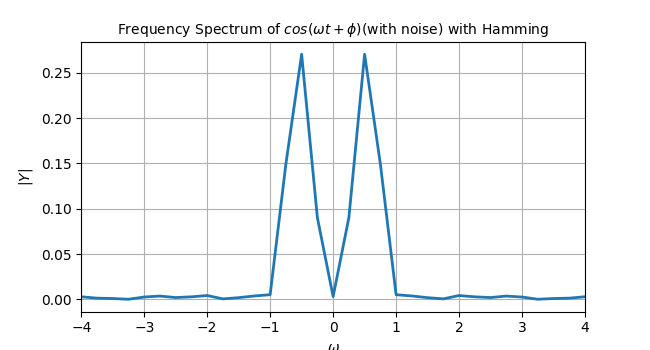
\includegraphics[scale=0.8]{Figure_20.png} 
	\label{fig:rawdata}
\end{center}
\clearpage

\begin{center}
	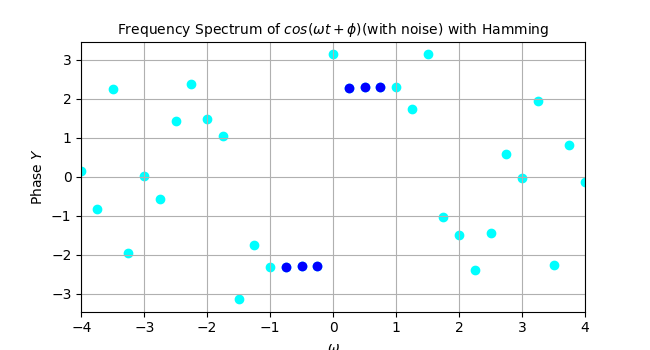
\includegraphics[scale=0.8]{Figure_21.png} 
	\label{fig:rawdata}
\end{center}
Similarly we try to estimate the frequency and phase by calculating weighted mean.
\begin{verbatim}
Estimations for cos(freq*t + phase) with noise without hamming:
Estimated frequency: 0.5
Estimated phase: 2.342789634255803

Estimations for cos(freq*t + phase) with noise with hamming:
Estimated frequency: 0.5585048423930653
Estimated phase: 2.294496634786052
\end{verbatim}

\section*{Frequency Spectrum of Chirped Signal $cos(16(1.5+ \frac{t}{2\pi})t)$}
This signal $cos(16(1.5+ \frac{t}{2\pi})t)$ is known as a \textbf{chirped signal}, since its frequency continuously changes from $16$ to $32$rad/s
\begin{verbatim}
def chirp(x):
    return cos(16*(1.5 + x/(2*pi))*x)

def hammingchirp(x):
    return chirp(x)*hammingFunction(arange(len(x)))
\end{verbatim}
we try to plot the DFT of this function from $t = -\pi$ to $\pi$ in $1024$ steps.
\clearpage

\begin{center}
	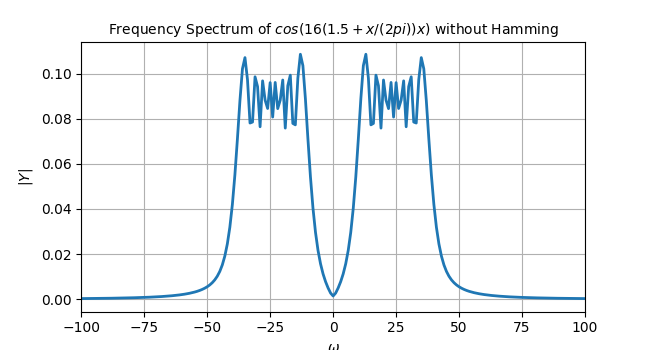
\includegraphics[scale=0.8]{Figure_22.png} 
	\label{fig:rawdata}
\end{center}
\begin{center}
	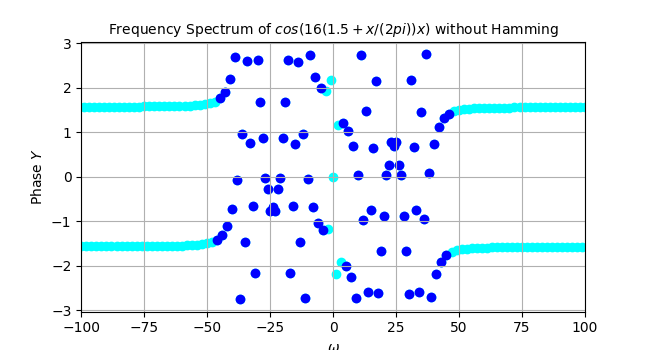
\includegraphics[scale=0.8]{Figure_23.png} 
	\label{fig:rawdata}
\end{center}
\begin{center}
	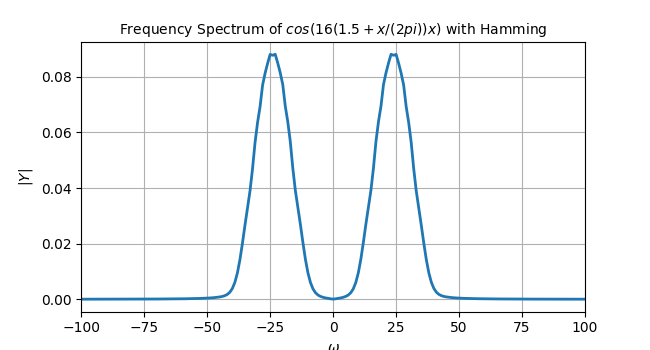
\includegraphics[scale=0.8]{Figure_24.png} 
	\label{fig:rawdata}
\end{center}
\clearpage

\begin{center}
	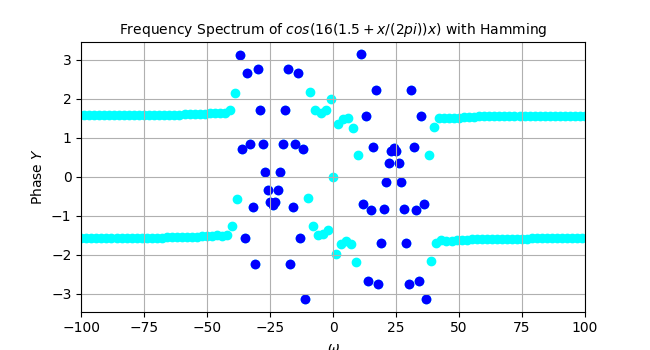
\includegraphics[scale=0.8]{Figure_25.png} 
	\label{fig:rawdata}
\end{center}
As expected the frequency of operation ranges from $16$ rad/s to $32$ rad/s. One can observe significant changes between the graphs with and without hamming. This is because the discontinuities have been removed to a great extend. The major frequencies are easily isolated and identifiable.
\\

The same $1024$ vector signal is broken into $16$ contiguous pieces of $64$ samples each to obtain the \textbf{Time Frequency Plot}. The DFT of each piece is obtained and stored in a 2D array. Each piece correspond to a different time interval. Plotting a surface plot with magnitude as a function of time and frequency using

\begin{verbatim}
w = linspace(-512, 512, 65)[:-1]
t = linspace(-pi, pi, 1025)[:-1]
t = reshape(t, (16, 64))
mag = []
phase = []

for time in t:
    y = chirp(time)
    y[0] = 0
    Y = fftshift(fft(fftshift(y)))/64
    mag.append(abs(Y))
    phase.append(angle(Y))

mag = array(mag)
phase = array(phase)
\end{verbatim}
If one closely observes, the gap between peaks increases with time
\clearpage
\begin{center}
	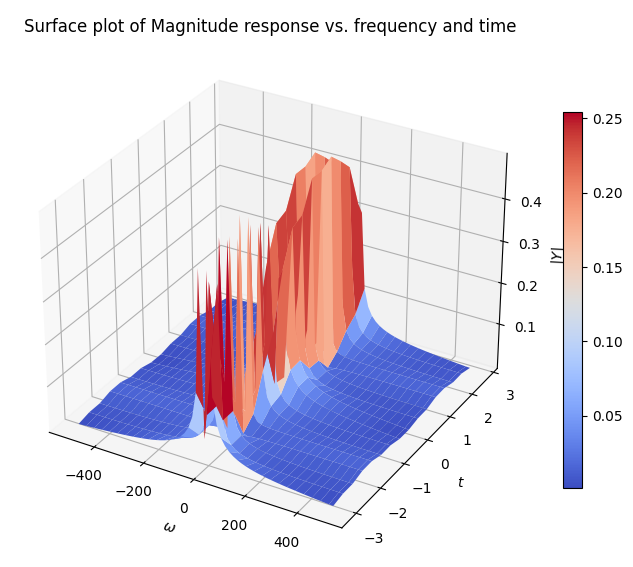
\includegraphics[scale=0.55]{Figure_26.png} 
	\label{fig:rawdata}
\end{center}

\begin{center}
	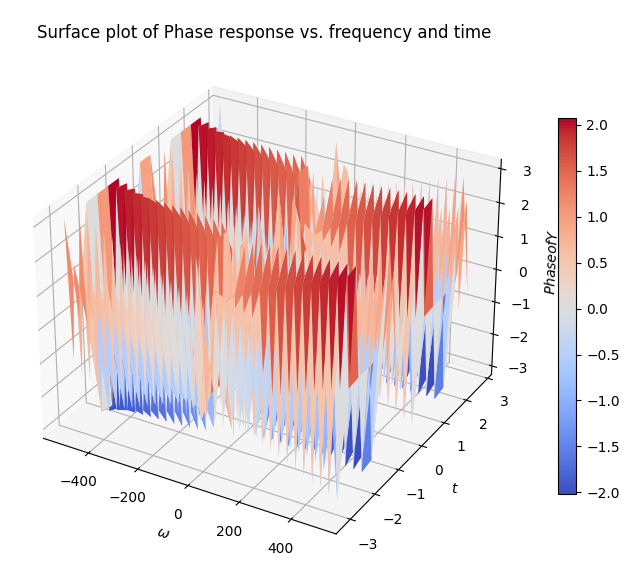
\includegraphics[scale=0.55]{Figure_27.png} 
	\label{fig:rawdata}
\end{center}
\clearpage
\begin{center}
	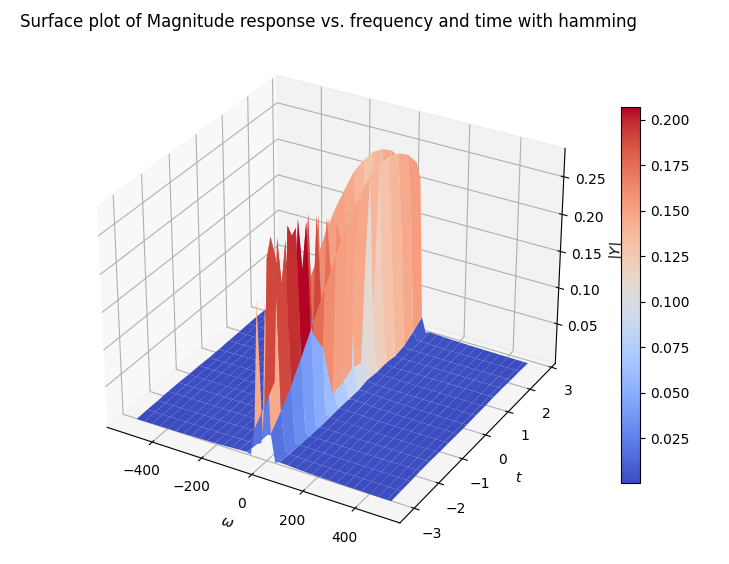
\includegraphics[scale=0.55]{Figure_28.png} 
	\label{fig:rawdata}
\end{center}

\begin{center}
	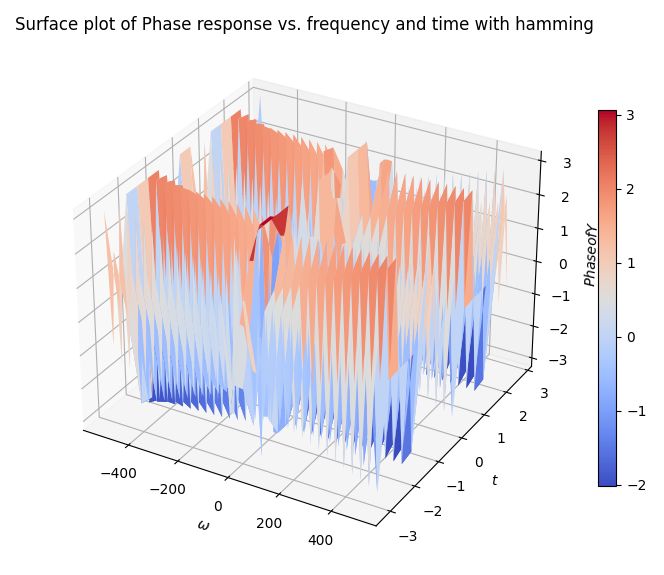
\includegraphics[scale=0.55]{Figure_29.png} 
	\label{fig:rawdata}
\end{center}
\clearpage

\section*{Conclusion}
Thus the frequency spectrum of non-periodic signals were analyzed and plotted. We observed how the discontinuities cause Gibbs Phenomenon and how it affects our DFT. By Windowing using Hamming technique, the effects of the discontinuities were reduced and well defined peaks were generated. We extracted the frequency and phase present in the signal by obtaining the weighted mean of the magnitudes. We also observed the time-frequency plot of a chirped signal to understand the time variation of DFT of a signal whose frequency continuously changes

\end{document}

